\chapter{Herramientas utilizadas}

En este capítulo se va a hacer una descripción de cada una de las herramientas utilizadas en el proyecto.

\section{Net2Plan}
\label{sec:net2plan}

Net2Plan \cite{net2plan} es una herramienta \textit{open-source} programada en Java dedicada a la planificación, optimización y simulación de redes de comunicaciones desarrollada por el grupo de investigación GIRTEL de la Universidad Politécnica de Cartagena. En sus inicios, fue concebida como una herramienta para docencia sobre redes de comunicaciones. Sin embargo, actualmente se ha convertido en una poderosa herramienta de optimización y planificación de redes, con un repositorio de recursos para la planificación de redes, tanto para el entorno académico como para el entorno de la industria y la empresa.

Net2Plan está basado en una representación de redes con componentes abstractos, tales como nodos, enlaces, demandas, ... Ésto está pensado para poder planificar cualquier tipo de red, sin importar la tecnología que utilice. Para poder personalizar las redes a gusto del usuario, cada componentes permite añadir atributos. Además, hay clases que permiten modelar una tecnología en concreto (redes IP, WDM o escenarios de NFV).

Net2Plan tiene dos modos de uso: mediante interfaz gráfica (GUI) y línea de comandos (CLI). La interfaz gráfica está pensada para utilizar en sesiones de laboratorio como un recurso formativo, o para poder ver más detalladamente la red sobre la que se está trabajando. Por otro lado, el modo línea de comandos facilita los estudios de investigación, ya que permite automatizar ejecuciones de algoritmos o simulaciones.
Como se ha hablado antes, ambos modos permiten utilizar Net2Plan en el entorno educativo (investigación o enseñanza) y en el entorno de la industria y la empresa.

\begin{figure}[ht!]
	\centering
	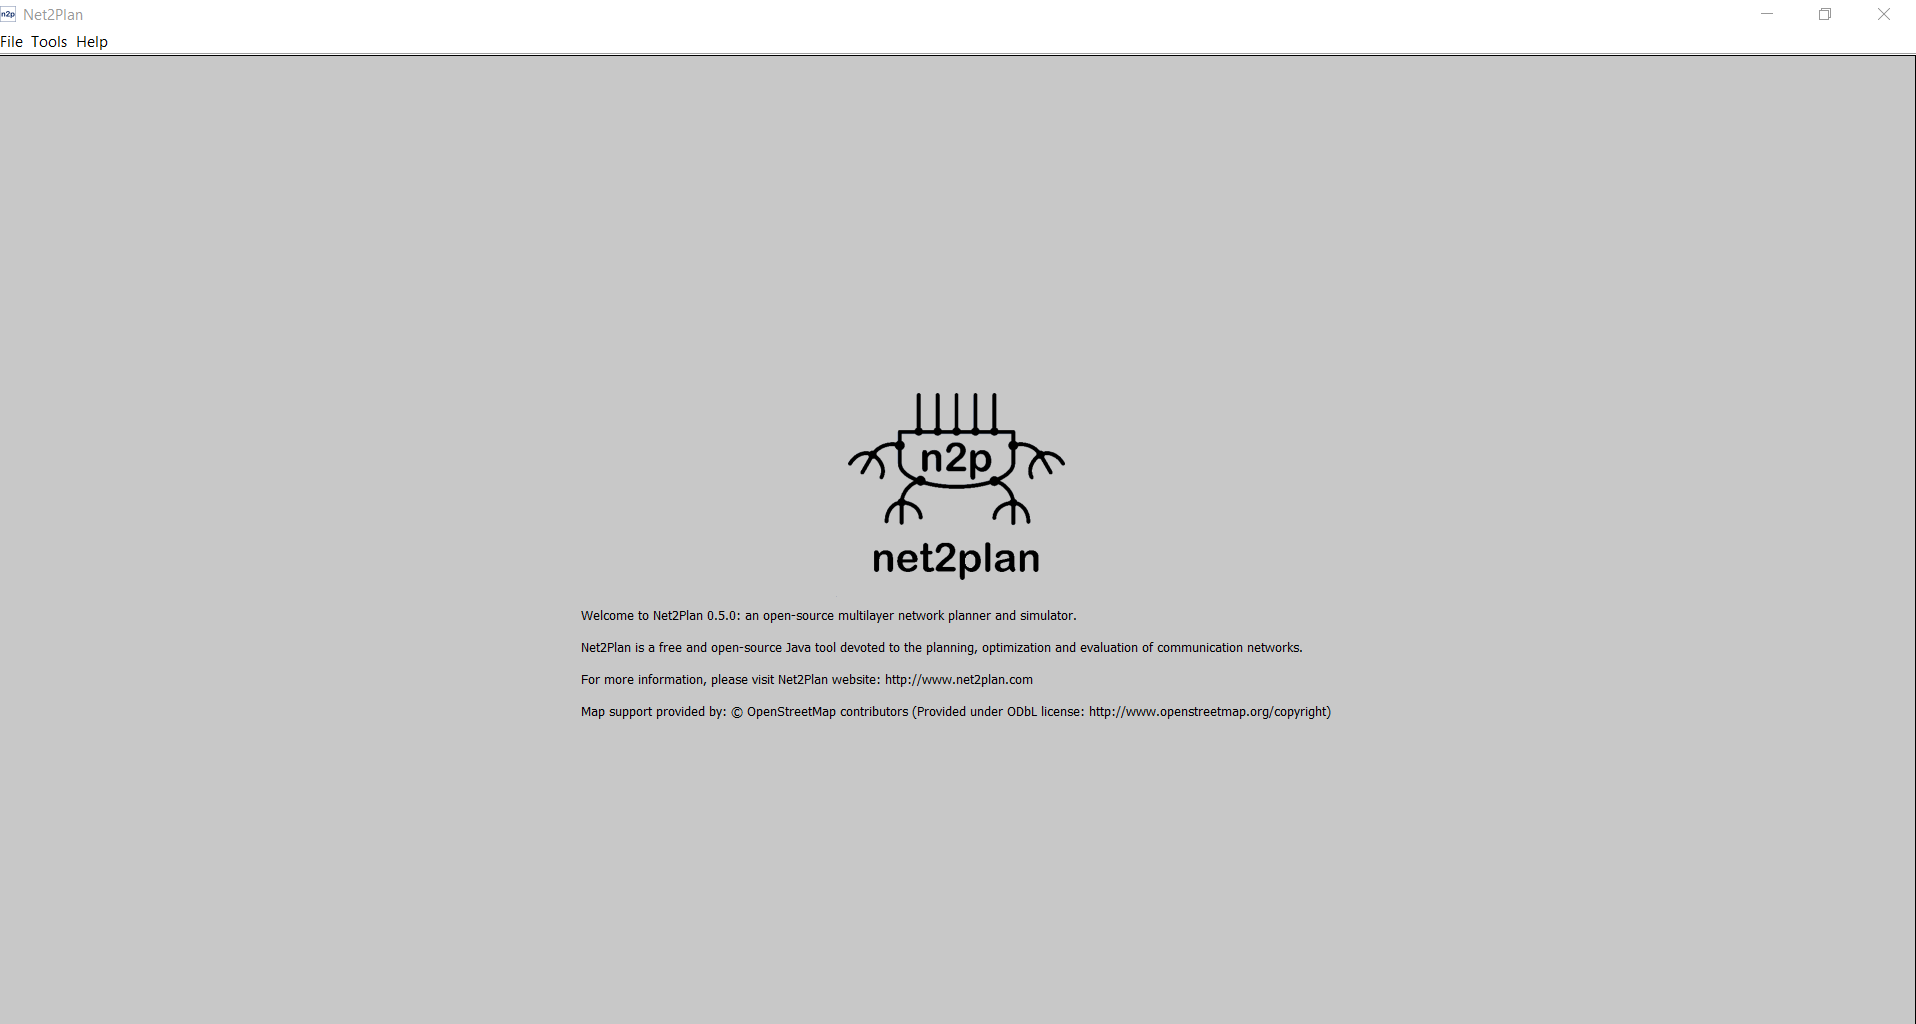
\includegraphics[width=1\linewidth]{imagenes/n2p_inicio}
	\caption{Ventana de inicio de Net2Plan}
	\label{fig:n2p_inicio}
\end{figure}
\begin{figure}[ht!]
	\centering
	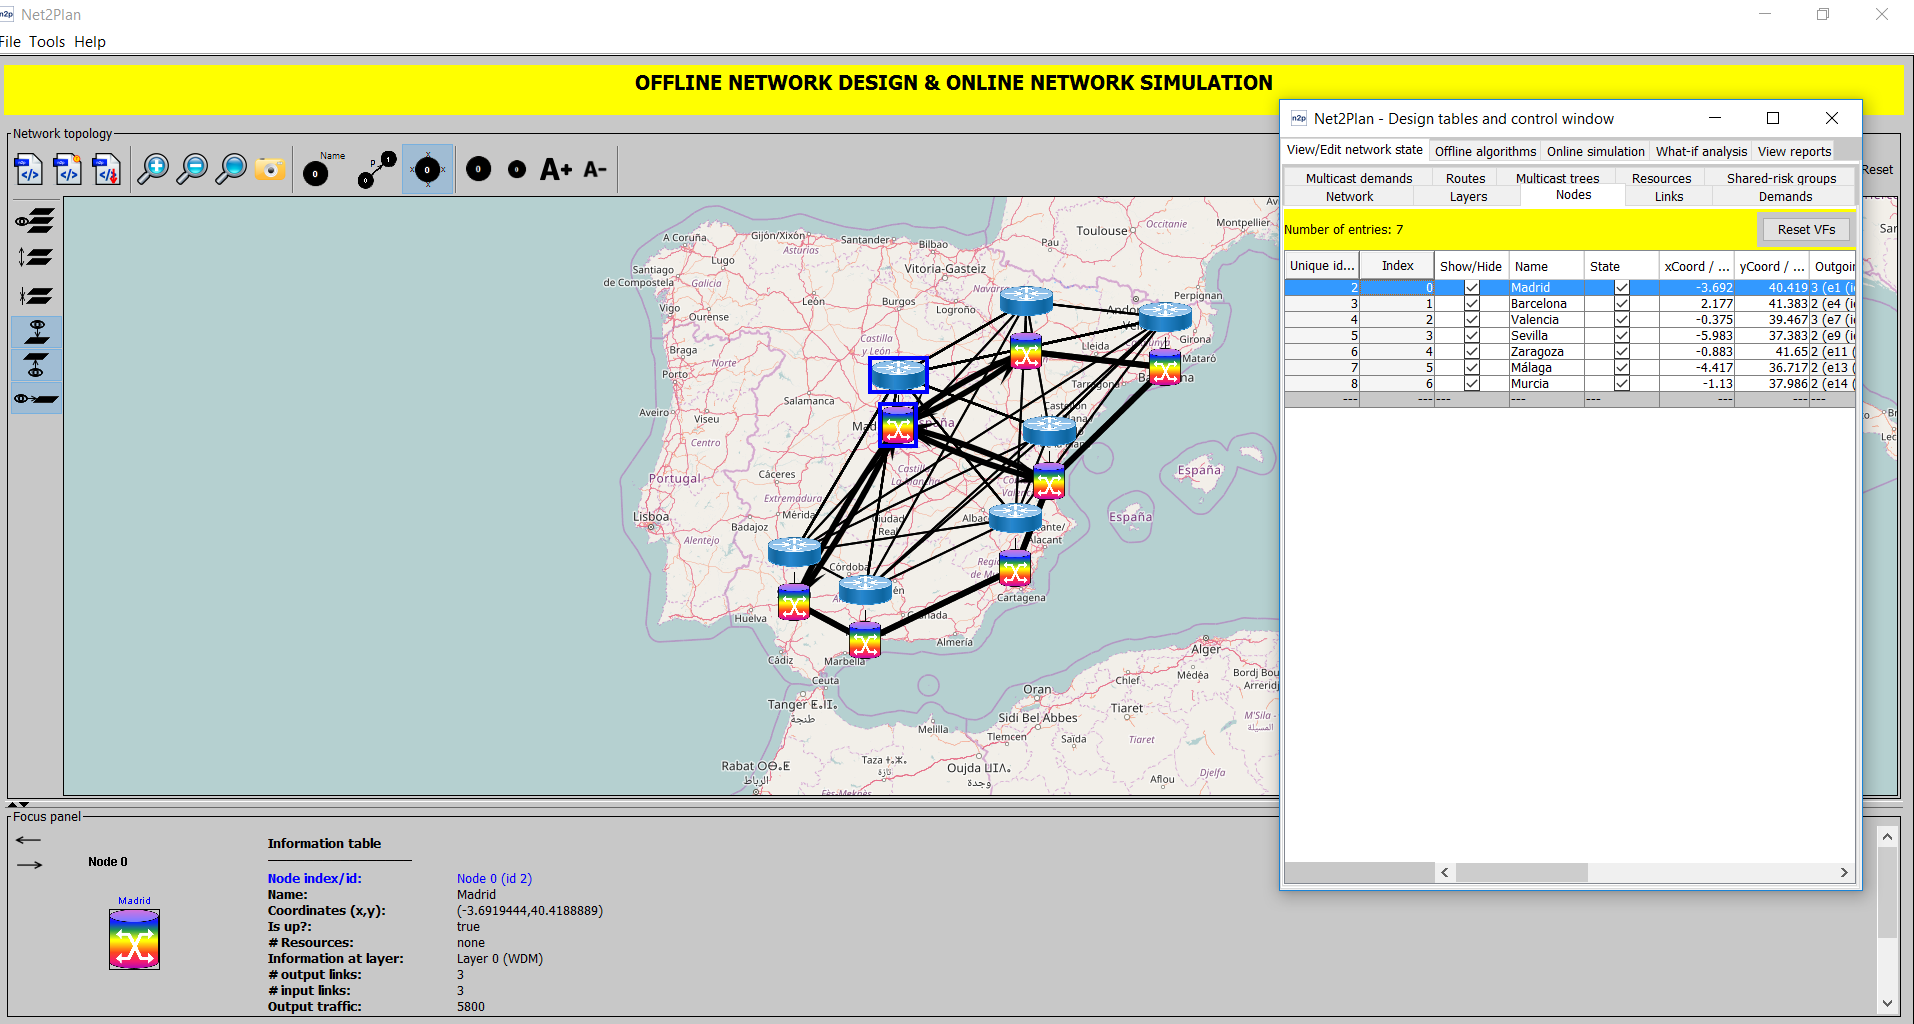
\includegraphics[width=1\linewidth]{imagenes/n2p_redes}
	\caption{Ventana \textit{Offline network desing and online network simulation}}
	\label{fig:n2p_redes}
\end{figure}
\clearpage

\section{Mininet}
\label{sec:mininet}

Mininet es una herramienta de emulación de redes que permite crear redes con \textit{hosts}, \textit{switches}, controladores y enlaces. Los \textit{hosts} de Mininet corren bajo un sistema operativo Linux, mientras que los \textit{switches} soportan el protocolo OpenFlow (ver \ref{subsec:openflow}) para mayor flexibilidad respecto a la configuración del \textit{routing} y para integrarlos dentro de un escenario SDN (ver \ref{sec:sdn}).

Mininet tiene una gran polivalencia, y eso permite que sea utilizado en diferentes tareas, tales como investigación, desarrollo, aprendizaje o testeo. Gracias a ello, se puede conseguir emular una red con un comportamiento similar a una real.

Sus principales características son:
\begin{itemize}
	\item Provee un amplio banco de pruebas para desarrollar aplicaciones basadas en OpenFlow.
	\item Permite que varios desarrolladores trabajen de forma concurrente sobre la misma topología de red.
	\item Permite realizar tests exhaustivos de topologías sin necesidad de tener una real.
	\item Incluye una Interfaz de Línea de Comandos que es independiente de la topología emulada y del protocolo que ésta utilice.
	\item Permite crear desde topologías mas sencillas con un único comando hasta topologías realmente complejas haciendo uso de una API de Python para definir los componentes con total detalle.
\end{itemize}

Las redes emuladas por Mininet ejecutan aplicaciones estandarizadas de Linux, como el kernel del propio sistema Linux. Esto permite que cualquier desarrollo llevado a cabo y testeado en Mininet pueda ser movido a un sistema real realizando las mínimas modificaciones posibles.

\section{ONOS}
\label{sec:onos}

ONOS (Open Network Operative System) es un proyecto Open-Source perteneciente a The Linux Foundation. Su principal objetivo es el de crear un controlador SDN para proveedores de servicios de comunicaciones.

Sus principales características son:
\begin{itemize}
	\item Escalabilidad: Ofrece replicación ilimitada mediante virtualización para poder añadir y quitar capacidad al plano de control según sea necesario.
	\item Alto rendimiento: Se ajusta perfectamente a las especificaciones de los operadores de red.
	\item Resistencia: Provee la disponibilidad requerida por los operadores de red.
	\item Retrocompatibilidad: Permite añadir o configurar dispositivos y servicios con configuración basada en modelos.
	\item Soporte a dispositivos de nueva generación: Ofrece control en real-time para dispositivos OpenFlow y, ahora también para dispositivos P4.
	\item Modularidad: Las funcionalidades de ONOS están definidas en modulos localizados, lo que hace más fácil probar y mantener el software en buen estado.
\end{itemize}


Está escrito en Java y opera como un clúster de nodos idénticos en cuanto al software. Trabaja con modelos y protocolos estandarizados, tales como OpenFlow (ver \ref{subsec:openflow}), NETCONF, OpenConfig, OpenROADM, ...


\begin{figure}[!ht]
	\centering
	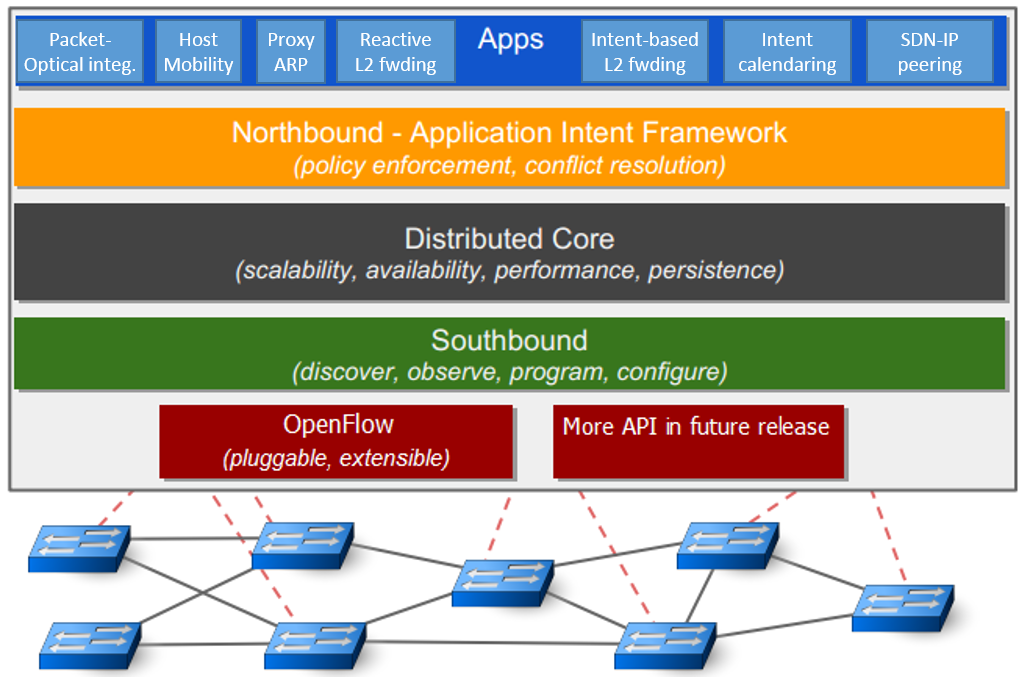
\includegraphics[width=0.6\linewidth]{imagenes/onos_architecture}
	\caption{Arquitectura de ONOS. 
		Fuente: http://sdnhub.org/tutorials/onos/}
	\label{fig:onosarch}
\end{figure}

En la figura \ref{fig:onosarch} se observa la arquitectura interna de ONOS. En el \textit{Core} se encuentran los controladores de los diferentes servicios que ofrece (TopologyService, DeviceService, HostService, ...), cada uno de ellos destinado a controlar un tipo de componente.

También se puede observar que, para acceder a estos controladores, las aplicaciones necesitan hacer uso de la interfaz \textit{NorthBound}, que se compone principalmente de una RestAPI.

Por otro lado, para que los controladores puedan tener constancia de los dispositivos de la red, la interfaz \textit{SouthBound} incluye diferentes \textit{drivers}, genéricos o particulares, para poder comunicarse con dispositivos mediante numerosos protocolos estandarizados, como se explicó anteriormente.

\clearpage

Para facilitar la interacción con el usuario, ONOS ofrece una GUI (ver figura \ref{fig:onosgui}) para ver en más detalle la topología que esta siendo gestionada, así como datos más específicos de cada uno de los dispositivos de la red. 

\begin{figure}[!ht]
	\centering
	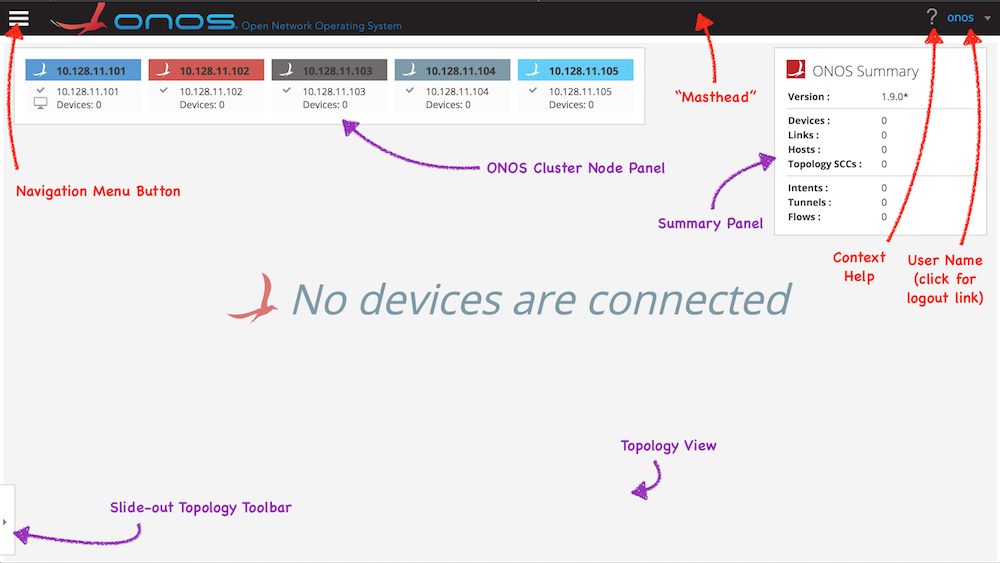
\includegraphics[width=0.8\linewidth]{imagenes/onos_gui}
	\caption{Interfaz Gráfica de ONOS. 
		Fuente: https://wiki.onosproject.org}
	\label{fig:onosgui}
\end{figure}

\subsection{OpenAPI}
\label{subsec:openapi}

OpenAPI es una iniciativa creada por varios expertos de la industria y la investigación para estandarizar las descripciones de las RestAPIs. Su principal objetivo es crear y promover un formato de descripción genérico.

Actualmente, prácticamente todas las aplicaciones utilizar APIs para conectarse con bases de datos, servicios y aplicaciones de terceros,... Gracias a la iniciativa de OpenAPI, las aplicaciones podrán conectarse entre sí de forma más rápida y sencilla, ayudando a tener un mundo realmente comunicado.

\section{OSM}
\label{sec:osm}

OSM (Open Source MANO) es un software \textit{open-source} cuya función principal es la orquestación de servicios de red avanzados en infraestructuras NFV heterogéneas. Surge como iniciativa de la ETSI para crear una arquitectura NFV común para los operadores de red.

OSM trabaja con una serie de componentes y conceptos que ayudan a definir su arquitectura:

\begin{itemize}
	\item \textbf{VDU (Virtual Deployment Unit):} Es el componente más básico de la arquitectura OSM. Se encarga de definir una máquina virtual. 
	
	\item \textbf{VLD (Virtual Link Descriptor):} Es el componente que se encarga de definir las conexiones entre diferentes componentes de la arquitectura. Hay principamente dos tipos de VLD: VDU-VDU y VNF-VNF.
	
	\item \textbf{VNFD (Virtual Network Function Descriptor):} Es el componente que se encarga de definir los recursos necesitados para instanciar un VNF. Incluye diferentes componentes: lista de VDUs, lista de VLDs, lista de conexiones,...
	
	\item \textbf{NSD (Network Service Descriptor):} Es el componente que se encarga de definir la información sobre la configuración de un NS. Incluye diferentes componentes: lista de VNFDs, lista de VLDs, parámetros de configuración iniciales, ...
	
	\item \textbf{VNF (Virtual Network Function):} Es el componente que define una función de red virtualizada. Ésta puede ser completa, cuando es una función realizada únicamente por él, o parcial, cuando es una función mas compleja que requiere de otros VNFs.
	
	\item \textbf{NS (Network Service):} Es el componente que se encarga de agrupar diferentes VNFs que realizan una función de red conjunta.
\end{itemize}

\begin{figure}[!ht]
	\centering
	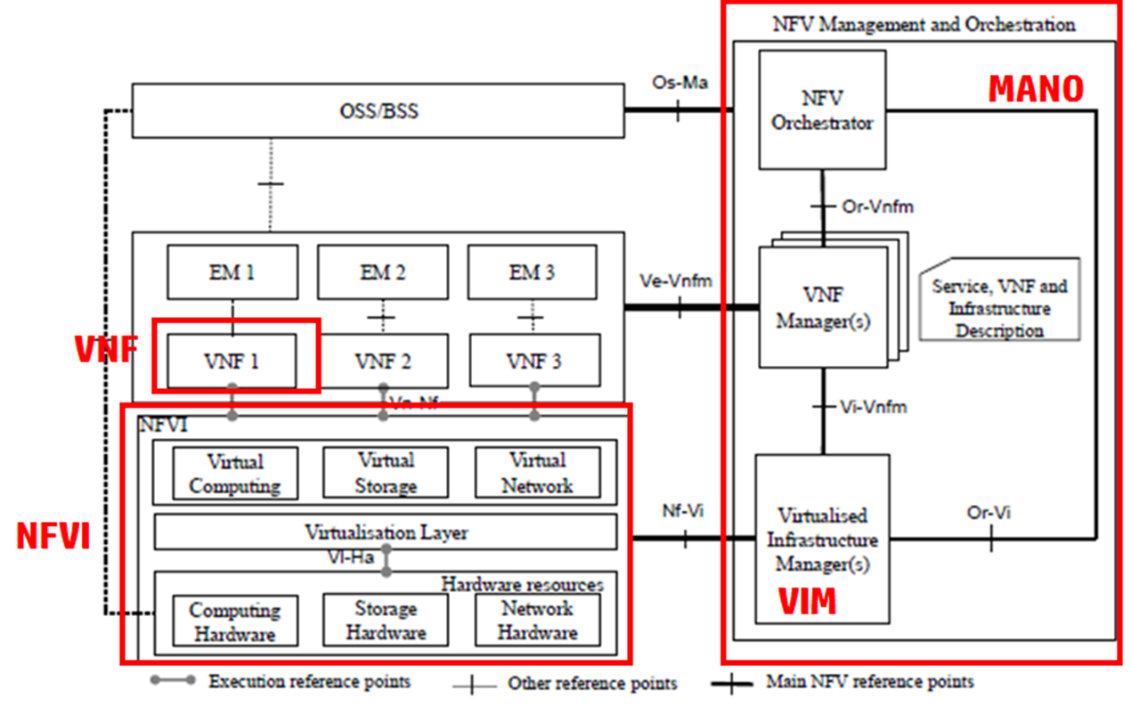
\includegraphics[width=0.8\linewidth]{imagenes/nfv_etsi_Arch}
	\caption{Arquitectura NFV de la ETSI. 
		Fuente: https://sdn.ieee.org/newsletter/july-2016/opensource-mano}
	\label{fig:nfvetsiarch}
\end{figure}

En la figura \ref{fig:nfvetsiarch} se puede ver un esquema de la arquitectura NFV que propone la ETSI, en la que se puede observar el papel que juega OSM en ella. 

\clearpage

\begin{figure}[!ht]
	\centering
	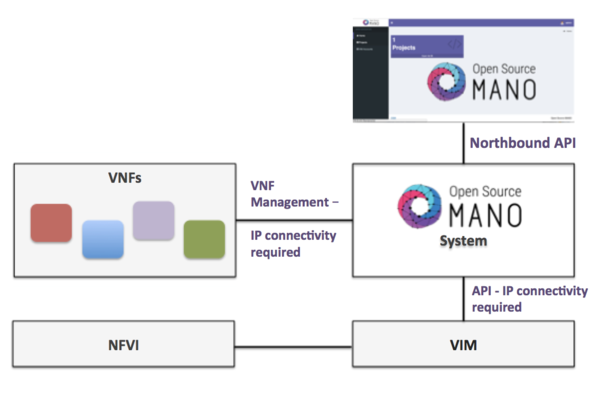
\includegraphics[width=0.8\linewidth]{imagenes/osm_arch}
	\caption{Arquitectura de OSM. 
		Fuente: https://osm.etsi.org/wikipub}
	\label{fig:osmarch}
\end{figure}

Para ayudar a explicar el funcionamiento de OSM, la figura \ref{fig:osmarch} da una visión general de la interaccion entre OSM y los diferentes componentes:

\begin{itemize}
	\item \textbf{Interfaz \textit{NorthBound}:} OSM exporta una RestAPI gracias a su interfaz \textit{NorthBound}. Mediante llamadas HTTP (GET, POST, DELETE), el usuario es capaz de ejecutar órdenes en OSM, tales como crear un nuevo VIM o instanciar un nuevo VNF, entre otras.
	
	Para ello, es necesario tener un cliente desde el cuál enviar órdenes. La ETSI ofrece una interfaz gráfica web que se instala al mismo tiempo que OSM y un cliente por línea de comando escrito en Python (\href{https://osm.etsi.org/wikipub/index.php/OsmClient}{OSMClient}).
	
	\item \textbf{Conexión con VIM:} OSM permite la comunicación con múltiples tipos de VIM (OpenStack, OpenVIM, VMWare y Amazon Web Services). Para ello, es necesaria conectividad IP entre OSM y el propio VIM, ya que las órdenes enviadas por OSM al VIM para realizar operaciones son hechas mediante una RestAPI.
	
	\item \textbf{Conexión VIM-NFVI:} NFV (NFV Infrastructure) es el conjunto de recursos (Memoria RAM, número de CPUs, Memoria de almacenamiento, ...) que son utilizados por un VIM para poder instanciar diferentes máquinas virtuales (VNFs). 
	
	En estructuras de trabajo pequeñas, es habitual que un VIM y su NFVI estén en la misma máquina física, aunque para estructuras reales de trabajo, la NFVI de un VIM puede estar distribuida en diferentes máquinas físicas.
	
	\item \textbf{VNF \textit{Management}:} cuando un VIM instancia un nuevo VNF, se le asigna una dirección IP para poder acceder a la propia máquina virtual y gestionarla. Por ello, es necesario que haya conectividad IP entre OSM y todos los VNFs. 
\end{itemize}

\clearpage

Una vez explicadas las interacciones que realiza OSM, se pueden explicar los pasos que sigue OSM para instanciar un nuevo NS en un determinado VIM:

\begin{itemize}
	\item \textbf{Paso 1.} Mediante la interfaz gráfica de OSM u otro cliente, el usuario escoge el NSD que quiere instanciar y en que VIM quiere hacerlo.
	
	\item \textbf{Paso 2.} OSM se pone en contacto con el VIM para ver si tiene todos los recursos necesarios para poder instanciar el NS.
	
	\item \textbf{Paso 3.} El VIM se pone en contacto con su NFVI para verificar si tiene todos los recursos necesarios. En caso afirmativo, todo continua de forma normal. En caso contrario, el VIM avisará a OSM de que no es posible llevar a cabo la instanciación.
	
	\item \textbf{Paso 4.} Una vez reservados los recursos necesarios, el VIM empieza a instanciar el NS. Esto toma un tiempo, ya que el VIM crea una instancia por VNF y tiene que aplicar todos los parámetros de configuración definidos en los descriptores.
	
	\item \textbf{Paso 5.} Cuando el NS ha sido instanciado satisfactoriamente, el VIM envía a OSM un mensaje de OK y desde OSM ya se pueden gestionar los diferentes VNFs pertenecientes al NS.
\end{itemize}


\section{OpenStack}
\label{sec:openstack}

OpenStack es una arquitectura basada en el paradigma \textbf{Cloud Computing} para controlar y gestionar grandes cantidades de recursos de computación, almacenamiento y red a través de un \textbf{Datacenter}. Para facilitar la gestión de recursos, OpenStack provee al usuario una interfaz gráfica a la vez que también exporta una RestAPI para permitir conectividad con aplicaciones externas.

\begin{figure}[!ht]
	\centering
	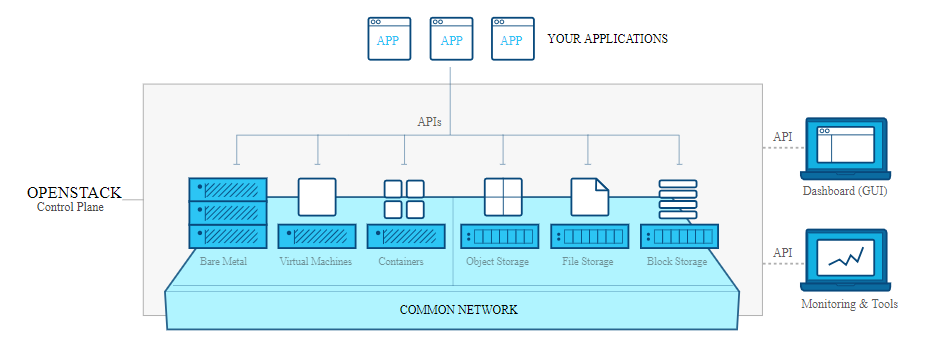
\includegraphics[width=0.9\linewidth]{imagenes/openstack_arch}
	\caption{Arquitectura de OpenStack. Fuente: https://www.openstack.org/software/}
	\label{fig:openstackarch}
\end{figure}

Está compuesto de diferentes bloques o módulos, encargándose cada uno de ellos de una funcionalidad concreta dentro de la arquitectura. Los módulos o servicios principales son los siguientes:

\begin{itemize}
	\item \textbf{Keystone:}  Este servicio controla la identificación de los diferentes usuarios que se conecten a la infraestructura de OpenStack, y el acceso a según que aplicaciones de los mismos.
	
	\item \textbf{Horizon:} Este servicio es el encargado de mostrar la gestión completa de OpenStack mediante una interfaz gráfica. Desde ella se puede observar con todo detalle que está sucediendo en el sistema y poder gestionar los posibles fallos.
	
	\item \textbf{Nova:} Este servicio está considerado el motor de OpenStack. Es el encargado de desplegar y administrar las diferentes máquinas virtuales instanciadas y otros servicios que se necesiten.
	
	\item \textbf{Neutron:} Este servicio es el encargado de que cada componente desplegado en OpenStack se comunique con los demas y estén interrelacionados.
	
	\item \textbf{Glance:} Este servicio se encarga de gestionar las diferentes imágenes que se usan en la infraestructura.
	
	\item \textbf{Cinder:} Este servicio se centra en el almacenamiento. Facilita el acceso al contenido alojado en las unidades de disco que se encuentren en la infraestructura.
	
	\item \textbf{Swift:} Este servicio es el encargado de almacenar los diferentes archivos del sistema, asegurar su integridad y replicarlos por los diferentes discos de la infraestructura, para hacer más dinámicas la accesibilidad y la disponibilidad.
\end{itemize}

\subsection{OpenStack4j}
\label{subsec:openstack4j}

OpenStack4j es un cliente \textit{open-source} programado en Java para controlar y gestionar un sistema basado en OpenStack.

\begin{figure}[!ht]
	\centering
	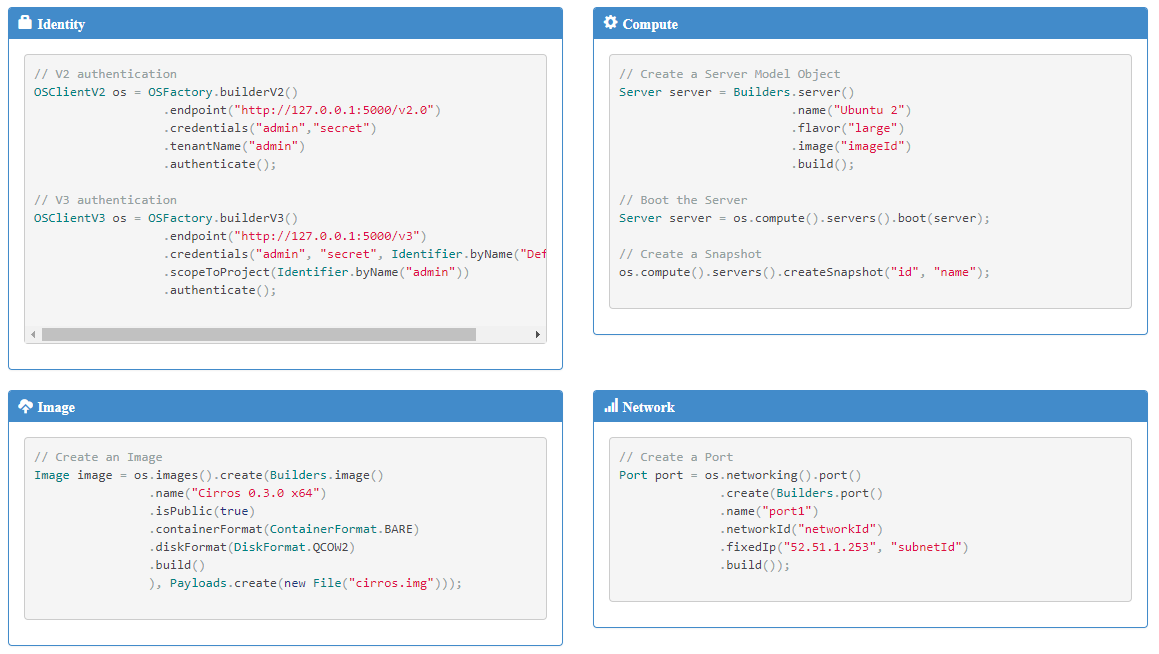
\includegraphics[width=0.8\linewidth]{imagenes/ejemplo_os4j}
	\caption{Ejemplo de OpenStack4j. Fuente: http://www.openstack4j.com/}
	\label{fig:ejemploos4j}
\end{figure}

